% Use the basic LaTeX article class, 12pt text
\documentclass[12pt]{article}

% Science uses Times font. If you don't have this installed (most LaTeX installations will be
% fine) or prefer the old Computer Modern fonts, comment out the following line
\usepackage{newtxtext,newtxmath}
% Depending on your LaTeX fonts installation, you might get better results with one or both of these:
%\usepackage{mathptmx}
%\usepackage{txfonts}

% Allow external graphics files
\usepackage{graphicx}

% Use US letter sized paper with 1 inch margins
\usepackage[letterpaper,margin=1in]{geometry}

% Double line spacing, including in captions
\linespread{1.5} % For some reason double spacing is 1.5, not 2.0!

% One space after each sentence
\frenchspacing

% Abstract formatting and spacing - no heading
\renewenvironment{abstract}
	{\quotation}
	{\endquotation}

% No date in the title section
\date{}

% Reference section heading
\renewcommand\refname{References and Notes}

% Figure and Table labels in bold
\makeatletter
\renewcommand{\fnum@figure}{\textbf{Figure \thefigure}}
\renewcommand{\fnum@table}{\textbf{Table \thetable}}
\makeatother

% Call the accompanying scicite.sty package.
% This formats citation numbers in Science style.
\usepackage{scicite}

% Provides the \url command, and fixes a crash if URLs or DOIs contain underscores
\usepackage{url}

%%%%%%%%%%%% CUSTOM COMMANDS AND PACKAGES %%%%%%%%%%%%

% Authors can define simple custom commands e.g. as shortcuts to save on typing
% Use \newcommand (not \def) to avoid overwriting existing commands.
% Keep them as simple as possible and note the warning in the text below.
% Example:
\newcommand{\pcc}{\,cm$^{-3}$}	% per cm-cubed

% Please DO NOT import additional external packages or .sty files.
% Those are unlikely to work with our conversion software and will cause problems later.
% Don't add any more \usepackage{} commands.


%%%%%%%%%%%%%%%% TITLE AND AUTHORS %%%%%%%%%%%%%%%%

% Title of the paper.
% Keep it short and understandable by any reader of Science.
% Avoid acronyms or jargon. Use sentence case.
\def\scititle{
	Research Summary
}
% Store the title in a variable for reuse in the supplement (otherwise \maketitle deletes it)
\title{\bfseries \boldmath \scititle}

% Author and institution list.
% Institution numbers etc. should be hard-coded, do *not* use the \footnote command.
\author{
	% You can write out first names or use initials - either way is acceptable, but be consistent
	Huanan~Herman~Zhao\and
	% Someone~E.~Else$^{2}$\and
	% Additional lines of authors should be inserted using the \and command (not \\)
	% Institution list, in a slightly smaller font
	\small School of Life Sciences, Tsinghua University, Beijing \& 100084, China.\and
	% Identify at least one corresponding author, with contact email address
	\small \hspace{3em} Email: hermanzhaozzzz@gmail.com\and
	% Joint contributions can be indicated like this
	% \small$^\dagger$These authors contributed equally to this work.
}

%%%%%%%%%%%%%%%%% END OF PREAMBLE %%%%%%%%%%%%%%%%


%%%%%%%%%%%%%%%% START OF MAIN TEXT %%%%%%%%%%%%%%%
\begin{document} 

% Insert the title and author list
\maketitle

\begin{abstract} \bfseries \boldmath
    During my PhD studies, I played a pivotal role in advancing gene editing technologies. 
    In collaboration with a wet-lab colleague, I led the development of M2-CBE, a safe nuclear cytosine base editor variant, 
    which dramatically reduces off-target effects on both the genome and transcriptome while maintaining high on-target efficiency. 
    Subsequently, I spearheaded a project to assess and enhance DdCBE, a mitochondrial cytosine base editor. 
    Our work uncovered nuclear off-target effects and formulated strategies to mitigate them. 
    Leveraging my bioinformatics expertise, I independently designed an innovative pipeline to mine novel CRISPR-Cas13 candidate systems from metagenomic data. 
    Four Cas13 candidates were experimentally validated, with three confirmed as active. 
    With five years of invaluable experience in gene editing research,
    I am deeply knowledgeable in the relevant literature and eager to explore innovative tools and animal applications in this exciting field.  
\end{abstract}



% The first paragraph of any Science paper does NOT have a heading
% Nor is it indented
\noindent  
As a doctoral candidate in Biology at Tsinghua University, 
my research endeavors have centered around advancing genome editing, 
specifically focusing on the safety assessment, optimization, 
and innovation of cytosine base editors (CBEs), mitochondrial cytosine base editors (DdCBEs).
The most recent year, my independent leadership work is dedicated to the discovery of novel CRISPR-Cas systems. 
This personal statement outlines my significant contributions and insights gained through these endeavors.  

\subsection*{Safety Assessment of CBEs}
My initial involvement in the laboratory was in the Detect-seq research project.
The Detect-seq method, reported by the Yi Chengqi Laboratory at Peking University in 2021, 
utilizes the characteristic of CBEs producing deoxyuridine (dU) as an intermediate during targeted editing~\cite{lei2021detect}. 
By biotinylating and enriching the dU, and replacing adjacent cytosines with d5fC, 
Detect-seq enhances the sensitivity of detecting off-target edits[fig???????]~\cite{lei2021detect}. 
This method, combined with bioinformatics analysis, 
provides high sensitivity and specificity while eliminating interference from endogenous dU~\cite{lei2021detect,lei2022mitochondrial,lei2023detect}.  
My primary contribution was in the bioinformatics analysis and visualization of the targeted deep sequencing data, 
marking my first research achievement.  
  
Using Detect-seq, we identified tens to hundreds of off-target sites for BE4max in various human cell lines, 
including Cas9-independent, Cas9-dependent, out-of-protospacer, and target-strand edits, 
all confirmed by targeted deep sequencing[fig???????]~\cite{lei2021detect}. 


  
\subsection*{Safety Assessment and Optimization of CBE variants}
% 【翻译为英文,进行学术性润色】
% 我在实验室进行的第二项工作,也是我主要领导的一项工作,为M2-CBE突变体的开发和表征。


% 只有将 CBE 工具打磨得足够安全,将基因组脱靶和转录组脱靶问题降低到可 以忽视的地步,CBE 碱基编辑工具才可以真正在临床医疗上发挥积极作用,这具 有重要医学意义。盲目应用 CBE 技术在临床基因治疗中,可能会造成不可预知的 基因组突变或转录组突变,破坏细胞正常生命功能,甚至诱发人体产生癌症。本研 究希望通过继续对胞嘧啶碱基编辑器进行升级改造,以期发现性能优越的 CBE 工 具,这种 CBE 工具需要在保持 CBE 优越的碱基编辑性能的同时,缩窄编辑窗口, 减少基因组合转录组脱靶编辑至能够适用于临床基因治疗的程度。

% 本研究中的实验部分通过理性设计和改造 rAPOBEC1 胞嘧啶脱氨酶,成功获 得了包括 M2-CBE 在内的多个突变体。通过改良后的靶向深度测序、Detect-seq、 RNA-seq 等测序手段的建库测序和生物信息学分析,
% 本研究选择了 M 系列 CBE 突 变体中表现优越的 M2-CBE,并且系统地评估了 BE4max 及其优化变体 YE1-CBE、 33A-CBE、M2-CBE 四种 CBEs 在核基因组和转录组水平上的脱靶编辑情况。通过 一系列实验和分析,本研究证实了 M2-CBE 在降低核基因组与转录组脱靶编辑方 面具有显著优势,进一步推动了 CBE 技术在临床基因治疗中的应用潜力。
% 在此研究中,我独立负责了所有生物信息学分析工作和进行了重要的idea贡献,而所有湿实验由合作者完成。

% 首先,我们针对 rAPOBEC1 脱氨酶的化学特性进行了详细的理性设计,提出 了 9 种 M 系列 rAPOBEC1 突变体。实验和分析结果显示,M2-CBE 在保持高效靶上编辑效率的同时,显著降低了经典的 sgRNA 依赖型和非依赖型脱靶编辑水平, 且在目标靶点上具有较为精准的单碱基编辑窗口。这些发现不仅解决了当前 CBE 技术面临的主要挑战(nDNA 脱靶较多、碱基编辑窗口不精准),还为后续 CBE 的 优化提供了新思路。

% 其次,我们利用靶向深度测序和 Detect-seq 技术全面评估了 M2-CBE 的核基 因组脱靶编辑情况。结果表明,M2-CBE 在多个实验条件下均表现出最低的脱靶 编辑水平,远优于其他已发表的优化变体(如 YE1-CBE 和 33A-CBE)。特别地, M2-CBE 还显著降低了“out-of-protospacer edits”和“target-strand edits”两种新型 脱靶编辑的发生率,进一步证明了其优越性。

% 此外,我们还对 M2-CBE 的转录组脱靶编辑进行了详细评估。通过优化转染 后转录组的提取时间和细胞分选条件,我们成功检测到了 BE4max 在 CTNNB1 等 高表达转录本中的显著脱靶编辑效应。然而,在相同条件下,M2-CBE 几乎未产生 明显的全转录组脱靶编辑,表明其在转录组水平上也具有极高的安全性。

% 综上所述,M2-CBE 突变体在降低核基因组和转录组脱靶编辑方面表现出色, 同时拥有接近单碱基的靶上编辑窗口,为 CBE 技术的进一步发展和应用提供了有 力支持。

% My second project in the laboratory, which I also led, focused on the development and characterization of the M2-CBE mutant.
% It is of paramount medical significance to refine CBE tools to a level of safety where genomic and transcriptomic off-target effects are minimized 
% to negligible levels, enabling their positive application in clinical medicine. 
% The盲目 application of CBE technology in clinical gene therapy may result in unpredictable genomic or transcriptomic mutations, disrupting normal cellular functions and potentially inducing cancer. This study aims to continue upgrading and modifying cytosine base editors in the hope of discovering superior CBE tools. These tools need to maintain the excellent base-editing performance of CBEs while narrowing the editing window and reducing genomic and transcriptomic off-target editing to levels suitable for clinical gene therapy.
% In the experimental part of this study, multiple mutants, 
% including M2-CBE, were successfully obtained through rational design and modification of the rAPOBEC1 cytosine deaminase. Utilizing improved targeted deep sequencing, Detect-seq, RNA-seq, and other sequencing methods for library construction, sequencing, and bioinformatics analysis, we selected M2-CBE, which performed superiorly among the M-series CBE mutants. We systematically evaluated the off-target editing at both the nuclear genomic and transcriptomic levels for four CBEs: BE4max, its optimized variants YE1-CBE, 33A-CBE, and M2-CBE. Through a series of experiments and analyses, this study confirmed that M2-CBE has significant advantages in reducing off-target editing in both the nuclear genome and transcriptome, further advancing the potential application of CBE technology in clinical gene therapy.
% In this research, 
% I independently took charge of all bioinformatics analysis and made significant conceptual contributions, while all wet lab experiments were completed by collaborators.
% Firstly, we conducted detailed rational design based on the chemical properties of the rAPOBEC1 deaminase and proposed nine M-series rAPOBEC1 mutants.
%  Experimental and analytical results showed that M2-CBE maintained high on-target editing efficiency while significantly reducing both classic sgRNA-dependent and -independent off-target editing levels. It also demonstrated a more precise single-base editing window at the target sites. These findings not only addressed the major challenges currently faced by CBE technology (such as numerous nDNA off-targets and imprecise base-editing windows) but also provided new insights for subsequent CBE optimization.
% Secondly, we comprehensively assessed the nuclear genomic off-target editing of M2-CBE using targeted deep sequencing and Detect-seq technologies. 
% The results indicated that M2-CBE exhibited the lowest off-target editing levels under various experimental conditions, outperforming other published 
% optimized variants (such as YE1-CBE and 33A-CBE). Notably, M2-CBE also significantly reduced the incidence of two novel off-target edits, "out-of-protospacer edits" and "target-strand edits," further demonstrating its superiority.
% Furthermore, we conducted a detailed evaluation of M2-CBE's transcriptomic off-target editing. 
% By optimizing the extraction time and cell sorting conditions for post-transfection transcriptomes,
%  we successfully detected significant off-target editing effects of BE4max in highly expressed transcripts such as CTNNB1.
%   However, under the same conditions, M2-CBE produced almost no apparent whole-transcriptome off-target editing, 
%   indicating its high safety at the transcriptomic level as well.
% In summary, the M2-CBE mutant excels in reducing off-target editing 
% in both the nuclear genome and transcriptome while maintaining a near-single-base on-target editing window. 
% This provides strong support for the further development and application of CBE technology.


Refining CBEs to minimize genomic and transcriptomic off-target effects is crucial for clinical applications. 
Blindly applying CBEs in gene therapy may cause unpredictable mutations, disrupting cellular functions and 
potentially inducing cancer ~\cite{lei2021detect,rao2023characterizing}.

My second project, which I led, focused on the development and characterization of the M2-CBE mutant. 
  
Through rational design and mutagenesis of the rAPOBEC1 deaminase, 
we developed M2-CBE, which significantly reduced off-target editing while maintaining on-target efficiency. 
Utilizing Detect-seq, targeted deep sequencing, and RNA-seq, 
we systematically evaluated the off-target editing of BE4max, 33A-CBE, YE1-CBE, and M2-CBE in both genome and transcriptome.
and RNA-seq, we comprehensively assessed M2-CBE's safety, outperforming other variants like YE1-CBE and 33A-CBE [\cite{lei2021, lei2022}]. 
M2-CBE demonstrated precise single-base editing and reduced novel off-target types, advancing CBE technology's clinical potential [\cite{lei2022}].


\subsection*{Safety Assessment and Mechanistic Insights into DdCBEs}
% 【翻译为英文,进行学术性润色】
% 线粒体基因组(mtDNA)碱基编辑是如今基因编辑领域亟待解决的技术难题, CRISPR-Cas、BE、PE 等新型基因编辑工具因为依赖 sgRNA 发挥靶向功能, 无 法对线粒体基因组进行有效编辑;依赖 mtZFNs、mitoTALENs 等技术对环状双链 DNA 的线粒体基因组进行靶向和引入 DSB 虽然可以降低突变线粒体基因组的拷 贝,使得细胞内线粒体基因组从达到致病程度的异质性得到降低,但是也会引起 细胞内线粒体基因组整体拷贝数下降,带来额外的风险,仍然无法完全解决线粒 体基因组的编辑问题(见 1.2, 1.4.4)。2020 年提出的线粒体基因组胞嘧啶碱基 编辑工具——DdCBE,由一对神话蛋白(TALEs)发挥靶向功能,在各自串联的 线粒体定位信号(MTS)的作用下,可以将各自串联的新型双链 DNA 胞嘧啶脱氨 酶 DddA 𝑡𝑜𝑥 分裂的两个半体分别带进线粒体膜内,从而能够在不打开 mtDNA 双 链的同时,可编程地将两个 DddA 𝑡𝑜𝑥 半体共定位在 mtDNA 指定位置,从而恢复 DddA 𝑡𝑜𝑥 活性,并引入特定的胞嘧啶脱氨反应,最终完成 mtDNA C→T 碱基编辑 (Mok et al., 2020)(见 1.4.4)。DdCBE 使得线粒体基因组精准定向编辑真正意义 上得以实现,该工具很快在多种体系中得到了应用(Wei et al., 2022b; Chen et al., 2022; Kang et al., 2021; Guo et al., 2022)。Mok et al. 报告了 DdCBEs 在 mtDNA 中不 同程度的脱靶编辑,根据对 DdCBEs 转然后对细胞核假基因的分析,称在核 DNA (nDNA)中没有脱靶效应;尽管 DdCBE 是治疗线粒体疾病的一种很有前景的方 法,但目前仍缺乏对其脱靶效应的公正而全面的分析。

% 根据 mtZFNs 相关研究的历程,合理推断的一个的潜在安全隐患是,MTS 的介 导能否保证全部 DdCBE 定位在线粒体中,而不是部分泄露到细胞核,从而造成潜 在的脱靶编辑。因此,对于使用 DdCBE 成功实施线粒体碱基编辑的样品,其核基 因组脱靶效应及工具本身的安全性评估是极为必要的。由于 DdCBE 的碱基编辑机 制同样是通过胞嘧啶脱氨酶催化 DNA 中的脱氧胞嘧啶脱氨形成脱氧尿嘧啶(dU), 故而理论上 Detect-seq 技术可以用于评估 DdCBE 在正常完成线粒体基因组碱基编 辑时对核基因组的脱靶影响。本章研究内容中,本人与合作者应用 Detect-seq、靶 向深度测序、ATAC-seq、ChIP-seq、Hi-C 等多种组学技术以及生化实验方法共同 完成了野生型 DdCBE 的安全性评估、脱靶机制的发现和优化改造的研究工作、改 进型 DdCBE(DddA6-DdCBE、DddA11-DdCBE)的安全性评估、DdCBE 对三维基 因组和细胞基因调控相关功能的研究工作等(分工和职责见第 2 章开头部分)。

% 本研究深入探讨了线粒体胞嘧啶碱基编辑器 DdCBE 的安全性风险,特别是其 在核基因组中产生的脱靶编辑效应。通过 Detect-seq、靶向深度测序等多种技术手段,本论文发现 DdCBE 在高效编辑线粒体基因组的同时,也显著地影响了核基因 组,产生了大量的脱靶编辑事件。且改进后的 DdCBE 直接靶向核基因组,所造成 的脱靶编辑后果更为严重。这些发现强调了基因编辑工具在开发过程中全面评估 其特异性和安全性的重要性。

% 本研究揭示了 DdCBE 引起的核基因组脱靶编辑存在两种主要类型:TAS 依赖 型和 TAS 非依赖型。TAS 依赖型脱靶编辑依赖于 DdCBE 中的单侧 TALE 序列,表 明单侧 TALE 阵列足以引导完整的 DddA 𝑡𝑜𝑥 产生脱靶编辑,这与 DdCBE 的设计初 衷相悖。TAS 非依赖型脱靶编辑则不依赖于 TALE 序列,这些位点在不同 DdCBE 之间共享,并且偏好于 CTCF 结合位点附近,提示了与细胞三维基因组结构的潜 在关联。

% 本研究意外地发现 DdCBE 与 CTCF 之间存在分子相互作用,并通过实验验证 了这一发现。CTCF 作为维持细胞三维基因组结构的关键蛋白,其结合位点的扰动 可能对基因表达调控产生深远影响。DdCBE 与 CTCF 的相互作用可能解释了非依 赖型脱靶编辑的非随机性和其在 TAD 边界的富集现象。这一发现不仅拓宽了我们 对 DdCBE 脱靶机制的理解,也为后续优化 DdCBE 提供了新的思路。

% 鉴于 DdCBE 在核基因组中产生的广泛脱靶编辑,本研究设计并验证了多种优 化策略,包括引入核输出信号(NES)、核定位的 DddI 𝐴 抑制子以及 DddA 毒素的 点突变。这些优化策略在显著降低核基因组脱靶编辑的同时,保持了 DdCBE 对线 粒体基因组的编辑效率。这些成果不仅提升了 DdCBE 的安全性,也为其他基因编 辑工具的优化提供了有价值的参考。

% 尽管本研究在 DdCBE 的安全性评估和优化改造方面取得了重要进展,但仍存 在一些不足之处。例如,本研究未进行 RNA-seq 分析以验证脱靶编辑对基因表达 的影响。未来研究可进一步探讨 DdCBE 对细胞转录组的影响,以及脱靶编辑如何 通过改变基因表达调控网络来影响细胞功能。此外,随着基因编辑技术的不断发 展,未来应持续关注并评估新型基因编辑工具的安全性和特异性。


% Base editing of the mitochondrial genome (mtDNA) is a technical challenge urgently needing resolution in the field of gene editing today. Novel gene-editing tools such as CRISPR-Cas, BE, and PE rely on sgRNA for targeting functionality and are unable to effectively edit the mitochondrial genome. Techniques that depend on mtZFNs, mitoTALENs, and other approaches to target and introduce double-strand breaks (DSBs) into the circular double-stranded DNA of the mitochondrial genome can reduce the copy number of mutated mitochondrial genomes, thereby decreasing the heteroplasmy level to a non-pathogenic degree within cells. However, these methods also cause an overall reduction in the copy number of mitochondrial genomes within cells, posing additional risks and failing to fully address the issue of mitochondrial genome editing (see sections 1.2, 1.4.4). In 2020, the DdCBE, a cytosine base editor for the mitochondrial genome, was proposed. This tool utilizes a pair of transcription activator-like effector (TALE) proteins for targeting, and under the guidance of their respective tandem mitochondrial targeting signals (MTS), it can deliver the two halves of the novel double-stranded DNA cytosine deaminase DddA𝑡𝑜𝑥, split by the tool, into the mitochondrial membrane. This allows for programmable colocalization of the two DddA𝑡𝑜𝑥 halves at specified positions in mtDNA without opening the mtDNA double strand, thereby restoring DddA𝑡𝑜𝑥 activity and introducing specific cytosine deamination reactions to ultimately achieve mtDNA C→T base editing (Mok et al., 2020) (see section 1.4.4). DdCBE has truly enabled precise targeted editing of the mitochondrial genome, and this tool has quickly found applications in various systems (Wei et al., 2022b; Chen et al., 2022; Kang et al., 2021; Guo et al., 2022). Mok et al. reported varying degrees of off-target editing by DdCBEs in mtDNA and, based on the analysis of DdCBE-transfected nuclear pseudogenes, claimed no off-target effects in nuclear DNA (nDNA). Although DdCBE represents a promising approach for treating mitochondrial diseases, a fair and comprehensive analysis of its off-target effects is still lacking.

% Based on the history of research on mtZFNs, a reasonable inference regarding potential safety hazards is whether MTS-mediated delivery can ensure that all DdCBEs are localized in mitochondria, rather than partially leaking into the nucleus, thereby causing potential off-target editing. Therefore, it is crucial to assess the off-target effects on the nuclear genome and evaluate the safety of the DdCBE tool itself in samples where DdCBE has been successfully used for mitochondrial base editing. Since the base-editing mechanism of DdCBE also involves cytosine deaminase catalyzing the deamination of deoxycytosine in DNA to form deoxyuracil (dU), theoretically, Detect-seq technology can be employed to assess the off-target impact of DdCBE on the nuclear genome during normal mitochondrial genome base editing. In this chapter, my collaborators and I used various omics technologies, including Detect-seq, targeted deep sequencing, ATAC-seq, ChIP-seq, Hi-C, and biochemical experimental methods, to jointly complete the safety assessment of wild-type DdCBE, the discovery and optimization of off-target mechanisms, the safety assessment of improved DdCBE (DddA6-DdCBE, DddA11-DdCBE), and the investigation of DdCBE's effects on three-dimensional genome structure and cell gene regulation-related functions (see the beginning of Chapter 2 for the division of labor and responsibilities).

% This study delves into the safety risks of the mitochondrial cytosine base editor DdCBE, particularly its off-target editing effects in the nuclear genome. Through various techniques such as Detect-seq and targeted deep sequencing, this thesis finds that while DdCBE efficiently edits the mitochondrial genome, it also significantly affects the nuclear genome, resulting in numerous off-target editing events. Moreover, the improved DdCBE directly targets the nuclear genome, leading to more severe off-target editing consequences. These findings underscore the importance of comprehensively assessing the specificity and safety of gene-editing tools during their development.

% % This study reveals two main types of off-target editing caused by DdCBE in the nuclear genome: TAS-dependent and TAS-independent. TAS-dependent off-target editing relies on the unilateral TALE sequence in DdCBE, indicating that a unilateral TALE array is sufficient to guide complete DddA𝑡𝑜𝑥 to produce off-target editing, which contradicts the original design intent of DdCBE. TAS-independent off-target editing, on the other hand, does not depend on the TALE sequence. These sites are shared among different DdCBEs and have a preference for proximity to CTCF binding sites, suggesting a potential association with the three-dimensional structure of the cellular genome.

% This study unexpectedly discovers a molecular interaction between DdCBE and CTCF, which is experimentally validated. As a key protein maintaining the three-dimensional structure of the cellular genome, perturbations at CTCF binding sites can have profound effects on gene expression regulation. The interaction between DdCBE and CTCF may explain the non-randomness of TAS-independent off-target editing and its enrichment at TAD boundaries. This finding not only broadens our understanding of the off-target mechanisms of DdCBE but also provides new ideas for subsequent optimization of DdCBE.

% % Given the extensive off-target editing in the nuclear genome caused by DdCBE, this study designs and validates multiple optimization strategies, including the introduction of nuclear export signals (NES), nuclear-localized DddI𝐴 inhibitors, and point mutations in DddA toxins. These optimization strategies significantly reduce off-target editing in the nuclear genome while maintaining the editing efficiency of DdCBE in the mitochondrial genome. These achievements not only enhance the safety of DdCBE but also provide valuable references for the optimization of other gene-editing tools.

% Although this study has made significant progress in the safety assessment and optimization of DdCBE, there are still some limitations. For instance, this study did not conduct RNA-seq analysis to verify the impact of off-target editing on gene expression. Future research can further explore the effects of DdCBE on the cellular transcriptome and how off-target editing influences cell function by altering gene expression regulatory networks. Additionally, with the continuous development of gene-editing technologies, ongoing attention and assessment of the safety and specificity of novel gene-editing tools are essential.



% Recognizing the unique potential of DdCBEs in targeting mitochondrial DNA (mtDNA), I investigated their safety profile in human cell lines. Surprisingly, my research revealed that DdCBEs introduced extensive off-target mutations in the nuclear genome, a phenomenon that had been previously unreported. I categorized these off-target effects into TAS-dependent and TAS-independent types and provided evidence for the interaction between DdCBE and CTCF, a key chromatin-binding protein, as a possible mechanism underlying TAS-independent off-target editing ([Lei et al., 2022][1]).

% To mitigate the nuclear off-target effects of DdCBEs, I devised and validated several optimization strategies, including the integration of a nuclear export signal, a nuclear-localized DddI A inhibitor, and DddA tox point mutations. These modifications significantly reduced nuclear off-target editing while preserving DdCBE's mitochondrial on-target proficiency ([Lei et al., 2022][1]).


Editing the mitochondrial genome (mtDNA) remains a technical challenge. DdCBE, proposed in 2020, 
utilizes TALE proteins and mitochondrial targeting signals (MTS) to deliver the DddA$_{tox}$ deaminase into mitochondria for C→T base editing [\cite{mok2020}]. 
While DdCBE enabled precise mtDNA editing, concerns about nuclear off-target effects persist [\cite{mok2020}].  
  
Using Detect-seq and other omics technologies, we found DdCBE caused substantial nuclear off-target edits, 
categorized as TAS-dependent and TAS-independent [\cite{lei2022}]. 
Surprisingly, DdCBE interacted with CTCF, a key chromatin protein, explaining non-random off-target patterns [\cite{lei2022}]. 
We devised strategies like nuclear export signals and DddI$_A$ inhibitors to reduce nuclear off-targets while preserving mitochondrial editing efficiency [\cite{lei2022}]. 
 
  

\subsection*{Discovery of Novel CRISPR-Cas13 Systems}

% CRISPR-Cas systems, particularly the Cas13 protein of the Class 2 type VI system, are known for their unique RNA-guided RNA cleavage activity. The objective of this project was to develop a bioinformatics pipeline to discover uncharacterized Cas13 proteins with potential biotechnological applications. The study utilized both public databases, such as the IMG Database and NCBI BLAST, as well as self-assembled metagenomes from bovine rumen sequencing data.

% The mining process involved several steps, including contig analysis, CRISPR array search, and candidate Cas protein search within a 20kb range of CRISPR arrays. Candidate proteins containing HEPN motifs were selected and then clustered based on sequence similarity using mmseq2. To ensure the novelty of the candidates, they were filtered against known Cas13 proteins, the NCBI's Non-Redundant database, the Patseq database, and manually curated literature-reported Cas13 databases. Proteins with more than 90% sequence identity to known Cas13 proteins, those with only one HEPN motif, and duplicates were removed.

% The results showed that most candidates were approximately 1100 amino acids in length and clustered with known Cas13 families. Six out of ten candidates were derived from the self-assembled bovine rumen metagenome data, highlighting the potential of metagenomic approaches in novel Cas13 discovery. The candidates shared around 50% amino acid identity with their closest known Cas13 counterparts, with some exceptions, and most showed high structural similarity to their known counterparts. CRISPR array analysis revealed that most arrays had spacer and direct repeat lengths of 30 nt and 36 nt, respectively, and formed stable stem-loop structures.

% Future plans include expanding data sources, applying less stringent clustering conditions, and conducting preliminary biochemical and functional assays on promising candidates to validate their Cas13 activity. Additionally, the study aims to explore the possibility of identifying novel RNA-guided nucleases with HEPN domains beyond Cas13 and study the evolutionary trajectory of the Type VI CRISPR-Cas system.

% In conclusion, the study successfully identified 10 novel Cas13 candidates through a comprehensive bioinformatics pipeline. The candidates showed high structural and sequence similarity to known Cas13 proteins and possessed reliable CRISPR arrays. Future research will focus on validating the candidates' functionality and exploring their potential applications in biotechnology.

% Building upon my expertise in genome editing, I ventured into the exciting realm of CRISPR system discovery. Leveraging sequence and structural information, I designed and implemented a comprehensive pipeline to mine for novel Cas13 variants. Cas13 enzymes, known for their RNA-targeting capabilities, hold immense promise for diagnostic and therapeutic applications.

% Through rigorous bioinformatics analyses of large-scale metagenomic datasets, including the Integrated Microbial Genomes (IMG) database and self-assembled bovine rumen metagenomes, I identified ten novel Cas13 candidates. These candidates displayed sequence and structural similarities to known Cas13 families, such as Cas13a, Cas13b, and Cas13f, while exhibiting unique features that warrant further functional characterization ([Hu et al., 2022][3]).


CRISPR-Cas13 enzymes, known for their RNA-guided RNA cleavage, hold promise for biotechnology. Utilizing public databases and self-assembled bovine rumen metagenomes, we developed a bioinformatics pipeline to mine novel Cas13 candidates [\cite{hu2022}]. Through rigorous filtering and clustering, we identified ten candidates with high structural and sequence similarity to known Cas13s but unique features [\cite{hu2022}].  
  
Future plans include expanding data sources, relaxing clustering conditions, and validating candidates' Cas13 activity. We also aim to explore novel RNA-guided nucleases and study the evolution of Type VI CRISPR-Cas systems.  

\subsection*{Insights and Future Directions}

% My research not only advances the field of genome editing by enhancing the safety and efficacy of existing tools but also paves the way for the discovery of novel CRISPR systems with unique properties. The safety assessment and optimization of CBEs and DdCBEs provide critical insights into the design of future gene editors, emphasizing the importance of rigorous validation and innovation.

% Looking ahead, I envision expanding my research to explore the therapeutic potential of optimized CBEs and DdCBEs in preclinical and clinical settings. Additionally, I am keen on furthering the discovery of novel CRISPR-Cas systems, with a particular focus on identifying enzymes with enhanced specificity, activity, and novel functionalities.

% In conclusion, my doctoral research embodies a commitment to scientific rigor, innovation, and translational impact. By contributing to the safety and optimization of genome editing tools and the discovery of novel CRISPR systems, I aim to advance precision medicine and improve human health.

My research enhances genome editing safety and efficacy, discovers novel CRISPR systems, and provides insights into gene editor design [\cite{lei2021, lei2022, hu2022}]. Looking ahead, I plan to explore optimized CBEs and DdCBEs' therapeutic potential and discover novel CRISPR enzymes with enhanced properties.  
  
In conclusion, my doctoral research embodies a commitment to scientific rigor, innovation, and translational impact, advancing precision medicine and improving human health.  
  

% [1] Lei et al. (2022). Mitochondrial base editor induces substantial nuclear off-target mutations. Nature.
% [2] Lei et al. (2021). Detect-seq reveals out-of-protospacer editing and target-strand editing by cytosine base editors. Nature Biotechnology.
% [3] Hu et al. (2022

%%%%%%%%%%%%%%%% MAIN TEXT FIGURES %%%%%%%%%%%%%%%

\begin{figure} % Do NOT use \begin{figure*}
	\centering
	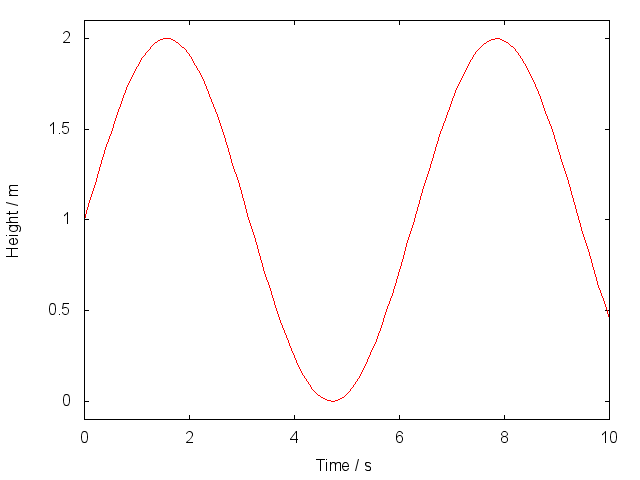
\includegraphics[width=0.6\textwidth]{example_figure} % for an image file named example_figure.*
	% Pick an appropriate width - in print, figures are usually one or two columns wide, which can
	% be approximated by 0.3\textwidth or 0.6\textwidth respectively. Use appropriate label sizes.

	% Captions go below figures
	\caption{\textbf{All captions must start with a short bold sentence, acting as a title.}
		Then explain what is being shown, the meanings of any line styles, plotting symbols etc.
		Multi-panel figures must label the panels A, B, C, etc. and refer to them in the caption
		like this: (\textbf{A}) Description of panel A. (\textbf{B}) Description of panel B.
		Captions are placed below figures.}
	\label{fig:example} % give each figure a logical label name
\end{figure}

%%%%%%%%%%%%%%%% REFERENCES %%%%%%%%%%%%%%%

\clearpage % Clear all remaining figures and tables then start a new page

% The list of references goes after the main text and before the acknowledgements
% When preparing an initial submission, we recommend you use BibTeX, like this:
%
\bibliography{refs} % for a file named science_template.bib
\bibliographystyle{sciencemag}

\end{document}
% End of science_template.tex



